% The turning-point failure, transverse plane.
% Track circle: centre c, radius R = pT/(0.3 B). Max reachable radius r_max = |c| + R.
% At T the tangent is purely azimuthal, so the straight-line extrapolation used by
% Surface::intersect aims at layers the track can NEVER reach, while the track
% curves back and re-crosses layers the Navigator has already retired.
\documentclass[border=8pt]{standalone}
\usepackage{tikz}
\usepackage{newtxtext,newtxmath}
\usetikzlibrary{arrows.meta,positioning,calc,backgrounds}

\begin{document}
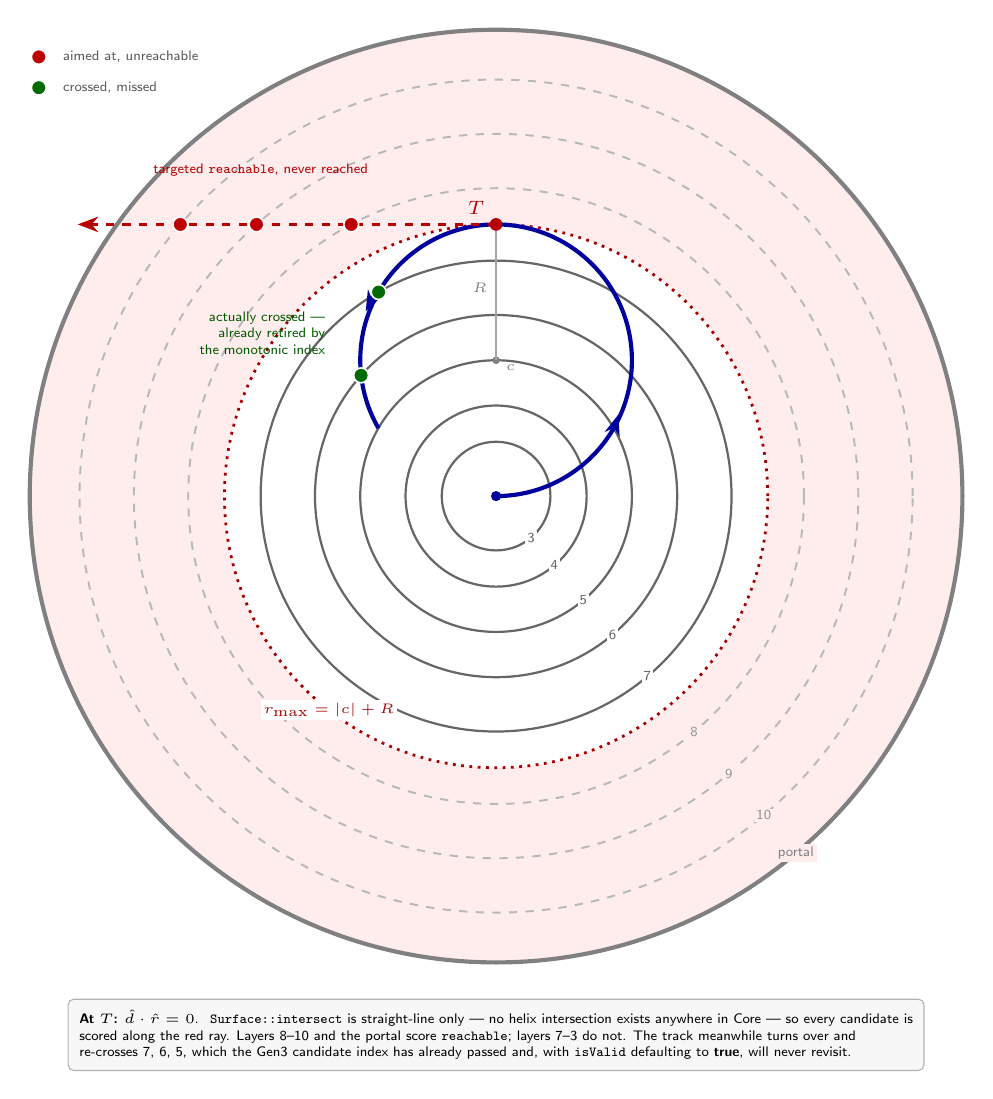
\begin{tikzpicture}[
  scale=1.15,
  font=\sffamily\footnotesize,
  reach/.style={draw=black!60,line width=0.8pt},
  unreach/.style={draw=black!28,line width=0.7pt,dashed},
  rmax/.style={draw=red!65!black,line width=1.0pt,dotted},
  portal/.style={draw=black!50,line width=1.5pt},
  track/.style={draw=blue!62!black,line width=1.5pt},
  tang/.style={draw=red!72!black,line width=1.1pt,dashed,-{Stealth[length=2.6mm]}},
  bad/.style={circle,fill=red!75!black,draw=white,line width=0.6pt,inner sep=1.9pt},
  good/.style={circle,fill=green!42!black,draw=white,line width=0.6pt,inner sep=1.9pt},
  lbl/.style={font=\sffamily\scriptsize},
  tny/.style={font=\sffamily\tiny}
]

% ---- unreachable region shading ----
\fill[red!7,even odd rule] (0,0) circle (5.15) (0,0) circle (3.0);

% ---- barrel layers ----
\foreach \r in {0.6,1.0,1.5,2.0,2.6} \draw[reach]   (0,0) circle (\r);
\foreach \r in {3.4,4.0,4.6}         \draw[unreach] (0,0) circle (\r);
\draw[portal] (0,0) circle (5.15);

% layer numbers along an empty diagonal
\foreach \r/\n in {0.6/3, 1.0/4, 1.5/5, 2.0/6, 2.6/7}
  \node[tny,text=black!60,fill=white,inner sep=0.7pt] at (-50:\r) {\n};
\foreach \r/\n in {3.4/8, 4.0/9, 4.6/10}
  \node[tny,text=black!42,fill=red!7,inner sep=0.7pt] at (-50:\r) {\n};
\node[tny,text=black!50,fill=red!7,inner sep=1pt] at (-50:5.15) {portal};

% ---- r_max envelope ----
\draw[rmax] (0,0) circle (3.0);
\node[tny,text=red!65!black,fill=white,inner sep=1pt] at (-128:3.0)
  {$r_{\max}=|c|+R$};

% ---- track ----
\draw[track] ([shift={(-90:1.5)}]0,1.5) arc[start angle=-90,end angle=210,radius=1.5];
\draw[track,-{Stealth[length=2.6mm]}] (1.30,0.74) -- (1.35,0.90);
\draw[track,-{Stealth[length=2.6mm]}] (-1.35,2.22) -- (-1.44,2.04);
\fill[blue!62!black] (0,0) circle (1.6pt);

% centre of curvature
\fill[black!50] (0,1.5) circle (1.2pt);
\node[tny,text=black!50,anchor=west,inner sep=1.5pt] at (0.06,1.42) {$c$};
\draw[draw=black!35,line width=0.5pt] (0,1.5) -- (0,3.0);
\node[tny,text=black!50,anchor=east,inner sep=1.5pt] at (-0.05,2.30) {$R$};

% ---- turning point ----
\fill[red!72!black] (0,3.0) circle (2.0pt);
\node[lbl,text=red!72!black,anchor=south east,inner sep=1.5pt] at (-0.08,3.06) {$T$};

% ---- tangent ray at T ----
\draw[tang] (0,3.0) -- (-4.62,3.0);

% ---- crossings targeted but unreachable ----
\foreach \x in {-1.600,-2.646,-3.487} \node[bad] at (\x,3.0) {};
\node[tny,text=red!72!black,anchor=south,align=center] at (-2.60,3.42)
  {targeted \texttt{reachable}, never reached};

% ---- re-crossings actually made ----
\foreach \x/\y in {-1.297/2.253, -1.491/1.333} \node[good] at (\x,\y) {};
\node[tny,text=green!35!black,anchor=east,align=right] at (-1.78,1.80)
  {actually crossed ---\\ already retired by\\ the monotonic index};

% ---- legend ----
\begin{scope}[shift={(-5.05,4.85)}]
  \node[bad]  at (0,0) {};
  \node[tny,anchor=west,text=black!65] at (0.16,0) {aimed at, unreachable};
  \node[good] at (0,-0.34) {};
  \node[tny,anchor=west,text=black!65] at (0.16,-0.34) {crossed, missed};
\end{scope}

% ---- caption ----
\node[draw=black!30,fill=black!3,rounded corners=2pt,inner sep=4pt,
      align=left,tny,anchor=north] at (0,-5.55)
  {\textbf{At $T$:} $\hat{d}\cdot\hat{r}=0$. \ \texttt{Surface::intersect} is straight-line only
   --- no helix intersection exists anywhere in Core --- so every candidate is\\
   scored along the red ray. Layers 8--10 and the portal score \texttt{reachable}; layers 7--3 do not.
   The track meanwhile turns over and\\
   re-crosses 7, 6, 5, which the Gen3 candidate index has already passed and,
   with \texttt{isValid} defaulting to \textbf{true}, will never revisit.};

\end{tikzpicture}
\end{document}
